\section{Kecerdasan Buatan}
\subsection{Definisi Kecerdasan Buatan}
 \hspace{1cm} Tahun 2020 salah satu stasiun televisi Korea menayangkan drama korea yang menjadi hype dan terkenal dengan judul "Start Up", lalu apa hubungannya dengan definisi dari kecerdasan buatan? didalam drama tersebut terdapat tokoh yang bernama Nam Do San , dia seoarang programmer sekaligus developer sebuah start up dimana dia membuat sebuah alat yang dinamakan dengan "NON GIL", alat ini dibuat untuk membantu orang buta dalam melakukan aktivitasnya dimana user akan memberikan beberapa statement yang sudah tercatat dalam database alat tersebut kemudian dijalan misal "NON GIL, bagaimana cuaca hari ini" atau " NON GIL siapakah yang berada didepan saya?" dengan statement tersebut alat ini bekerja layaknya manusia dan memberika jawaban spesifik seperti yang di minta oleh user. dari contoh diatas sudah ada bayang bayang tentang apa itu kecerdasan buatan.
 
\hspace{1cm}Selain itu, contoh sederhana penerapan kecerdasan buatan disekitar kita adalah SIRI, bagi pengguna IOS pasti sudah tidak asing dengan SIRI yang seringkali diartikan sebagai asisten pribadi pengguna IOS dalam melakukan hal hal tertentu untuk penggunanya. 

\hspace{1cm} Menurut John McCarthy(1956) Kecerdasan buatan adalah usaha memodelkan proses berpikir manusia dan mendesain mesin agar dapat menirukan perilaku manusia. dan masih banyak lagi ahli pendapat mengenai definisi dari kecerdasan buatan. namun kembali lagi pada secercah ceritita diatas, poin utamanya adalah bagaimana manusia menciptakan teknologi yang mampu berpikir seperti manusia itu sendiri itulah sederhananya definisi kecerdasan buatan atau dalma bahasa inggris Artificial Intellegent atau AI.

\subsection{Sejarah dan perkembangan Kecerdasan Buatan}
\hspace{1cm} Istilah kecerdasan buatan pertama kali dikemukakan pada tahun 1956 di Konferensi Darthmouth.Tokoh utama yang seringkali dikaitkan dengan AI adalah John McCarthy yang dimana dia mendefinisikan bahasa pemrograman LISP, yang sekarang sering digunakan dalam pembuatan program-pogram kecerdasan buatan dari hal tersebut dia membuat sebuah program yang disebut Programs with Common Sense.

\hspace{1cm} Selanjutnya Pada tahun 1959, Dari IBM ada seorang bernama Nathaniel Rochester bersama beberapa mahasiswa lainnya mengeluarkan program kecerdasan buatan yaitu Geometry Theorm Prover. Kemudian Pada tahun 1963, program yang  mampu menyelesaikan masalah integral tertutup untuk mata kuliah Kalkulus dibuat James Slagle. Selanjutnya Pada tahun 1986, program analogi yang digunakan dalam pemecahan masalah analogi geometris yang ada pada tes IQ dibuatan Tom Evan. Dari tahun 1980an AI kemudian mulai berkembang dibidang idustri dan mulai berkiprah hingga saat ini dimana para ilmuan berlomba lomba menciptakan AI yang bermanfaat untuk kehidupan sekarang atau dimasa depan nanti.

\subsection{Supervised learning dan Unsupervised Learning}
\hspace{1cm} Berbicara mengenai AI , didalam AI adapun yang disebut dengan Machine learning dimana akan dikategorikan berdasarkan label atau tag. Maksud dari tag atau label ini adalah lebih membahas tentang target variable apakah ada atau tidak dasar datanya. 
 
\hspace{1cm}Supervised learning   di mana datanya dilengkapi dengan atribut tambahan yang ingin kita prediksi dengan clasifiation dan regression. Classification adalah tentang sampel milik dua atau lebih kelas dan kita ingin belajar dari data yang sudah berlabel bagaimana memprediksi kelas data tak berlabel contoh klasifikasi atau clasification adalah pengenalan digit tulisan tangan, di mana tujuannya adalah untuk menetapkan setiap vektor masukan ke salah satu dari sejumlah kategori diskrit yang terbatas. dan regresi dimana jika keluaran yang diinginkan terdiri dari satu atau lebih variabel kontinu, maka tugas tersebut disebut regresi. Contoh masalah regresi adalah prediksi panjang salmon sebagai fungsi dari umur dan beratnya. Contoh sederhananya adalah pada gambar Sapi di tag “sapi” di tiap masing masing image sapi dan gambar kuda di tag “kuda” di tiap masing gambar kuda. Machine learning kategori dapat berupa clasification (“sapi”, “kuda”, “kambing”, dan lain sebagainya) dan regression ( berat badan, tinggi badan, umur , dan lain lain). Supervised learning banyak digunakan dalam memprediksi pola dimana pola tersebut sudah ada contoh data yang lengkap, jadi pola yang terbentuk adalah hasil pembelajaran data lengkap tersebut. 

\hspace{1cm} Jika Supervised learning tentang atribut atau label yang sudah ada dari kateogri yang diinginkan maka berbeda dengan unservised learning dimana dimana unsupervised menggunakan ke samaan dari attribut attribut yang dimiliki. Jika attribut dan sifat sifat dari data data feature yang diekstrak memiliki kemiripan, maka akan dikelompok kelompokan (clustering). Sehingga hal ini akan menimbulkan kelompok kelompok (cluster). Jumlah cluster bisa unlimited atau tidak terbatas.

\subsection{Data Set, Training Test, Testing Test}
\hspace{1cm} berbicara mengenai Supervised learning serta unsupervised learning maka harus adanya pembahasan mengenai definisi dataset. Dataset adalah kumpulan sampel yang sudah dikumpulkan. Seorang anak ingin bermain badminton, tetapi keputusannya untuk bermain badminton (play) tergantung pada variable yang ditentukan contohnya jarak kaki dari gairs dan atau tinggi net sehingga variable varibale ini disebut fitur.

\hspace{1cm} Sedangkan Training Test dan Testing set tentang mempelajari beberapa properti kumpulan data dan kemudian menguji properti tersebut terhadap properti lainnya Himpunan data. Praktik umum dalam pembelajaran mesin adalah mengevaluasi algoritma dengan membagi kumpulan data menjadi dua. Kita menyebut salah satu set itu sebagai Training Test, di mana kita mempelajari beberapa properti kita menyebut himpunan lain sebagai himpunan Testing Test, tempat kita menguji properti yang dipelajari.


\section{Instalasi}
Buka Link https://scikit-learn.org/stable/tutorial/basic/tutorial.html untuk mendapatkan source code yang akan digunakan 
\begin{enumerate}
    \item Instalasi library scikit dari anaconda dengan pip install -U scikit-learn, 
     \begin{center}
    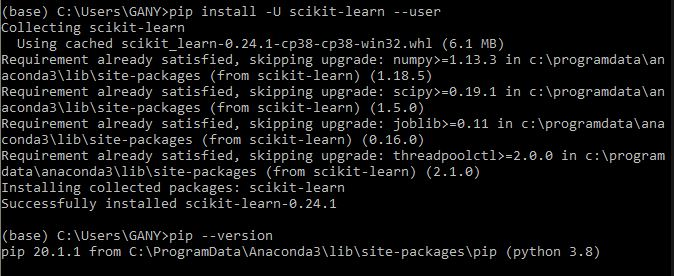
\includegraphics[width=.8\textwidth]{figures/1184008/chapter1/1.JPG}
    \end{center}
    \item Mencoba Loading an example dataset, dengan membuka link yang sudah tertera pada Main dan mengambil salah satu example dan jalankan spyder dan lihat hasilnya
     \begin{center}
     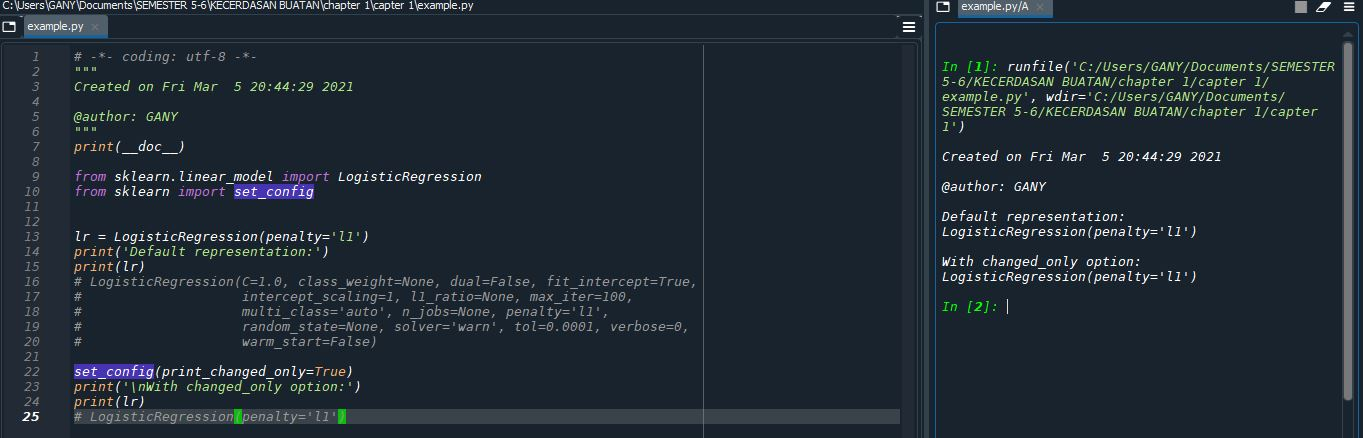
\includegraphics[width=.8\textwidth]{figures/1184008/chapter1/2.JPG}
     \end{center}
     SC : Example
     \begin{verbatim}
    from sklearn.linear_model import LogisticRegression
    from sklearn import set_config
    lr = LogisticRegression(penalty='l1')
    print('Default representation:')
    print(lr)
    set_config(print_changed_only=True)
    print('\nWith changed_only option:')
    print(lr)
    \end{verbatim}
     Hasil dari example
     \begin{center}
     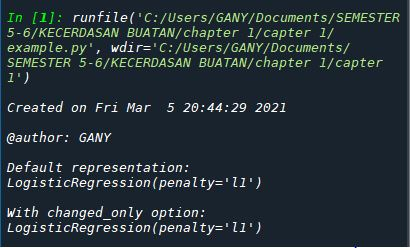
\includegraphics[width=.8\textwidth]{figures/1184008/chapter1/2a.JPG}
     \end{center}
     untuk datasetnya bisa dilihat pada link untuk source codenya
    \begin{center}
     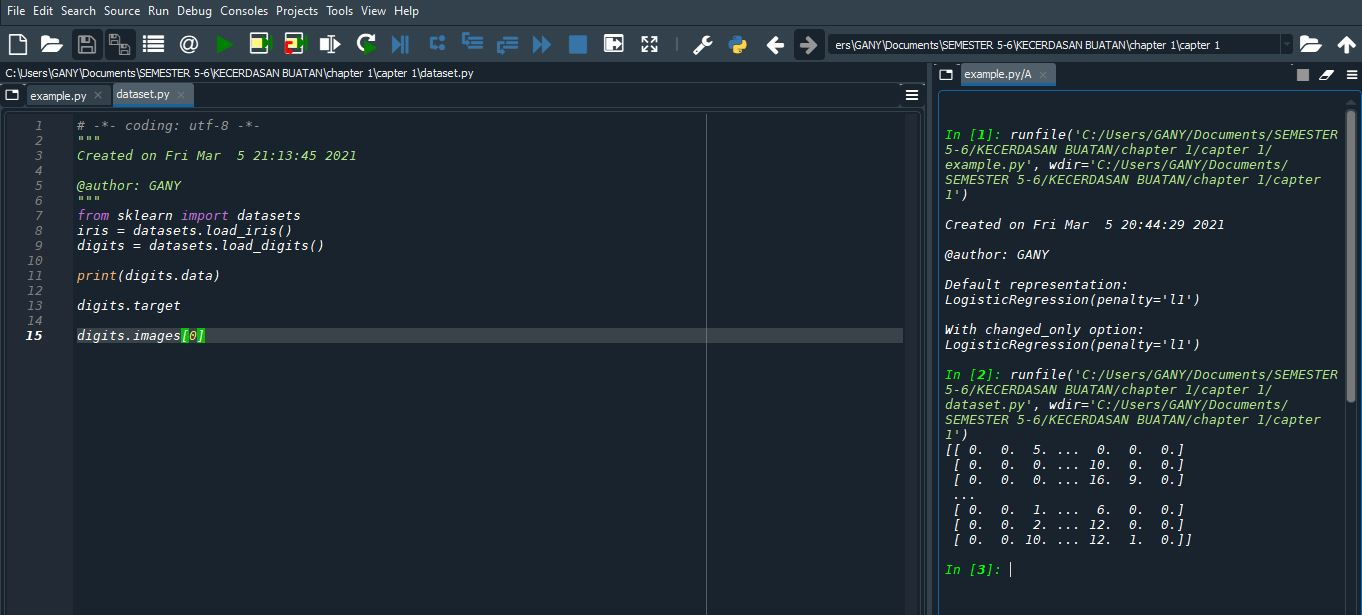
\includegraphics[width=.8\textwidth]{figures/1184008/chapter1/3.JPG}
    \end{center}
    SC : Dataseats
    \begin{verbatim}
    from sklearn import datasets 
    iris = datasets.load_iris()
    digits = datasets.load_digits()
    print(digits.data) 
    digits.target
    digits.images[0]    
    \end{verbatim}
    Hasil dari dataset
    \begin{center}
     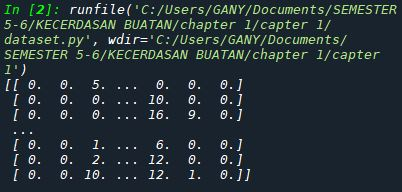
\includegraphics[width=.8\textwidth]{figures/1184008/chapter1/3a.JPG}
    \end{center}
    \item Mencoba Learning and predicting, dengan membuka link sebelumnya dan mencari learning dan predicting, lalu buat file baru pada spyder dan run
    \begin{center}
    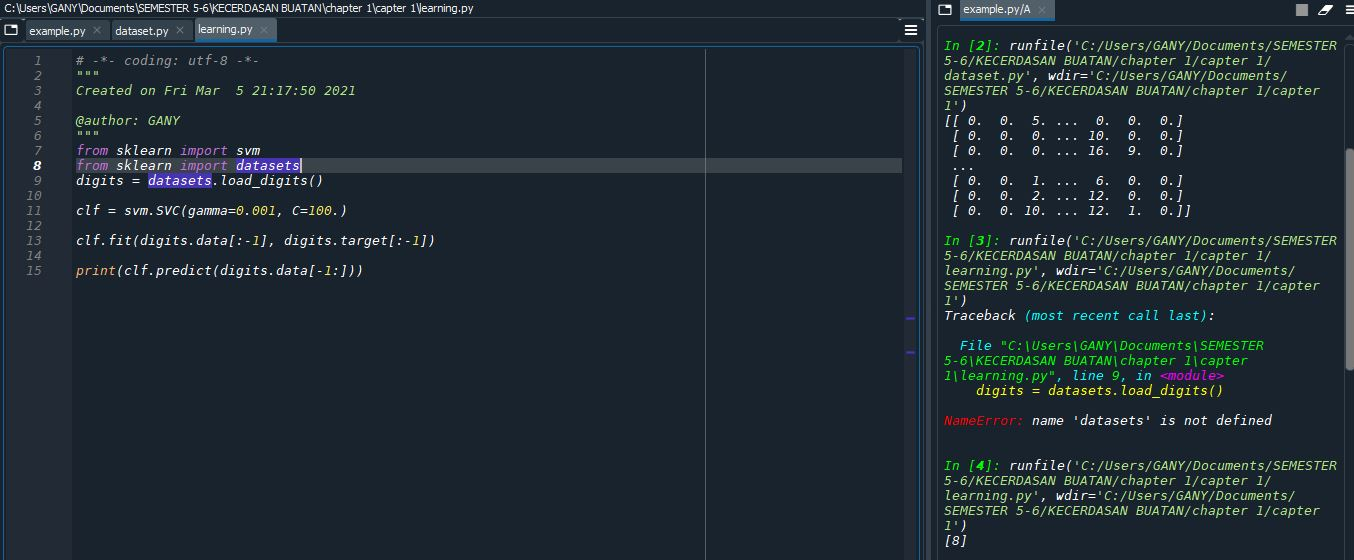
\includegraphics[width=.8\textwidth]{figures/1184008/chapter1/4.JPG}
    \end{center}
    SC : Learning and predicting
    \begin{verbatim}
    from sklearn import svm 
    from sklearn import datasets 
    digits = datasets.load_digits() 
    clf = svm.SVC(gamma=0.001, C=100.) 
    clf.fit(digits.data[:-1], digits.target[:-1])
    print(clf.predict(digits.data[-1:]))    
    \end{verbatim}
    Hasil dari learing predicting 
    \begin{center}
    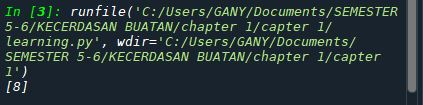
\includegraphics[width=.8\textwidth]{figures/1184008/chapter1/4a.JPG}
    \end{center}
    Yang kemudian akan tampak file JobLib pada folder yang sama dan jika dibuka pada notepad akan tampak seperti dibawah ini
     \begin{center}
    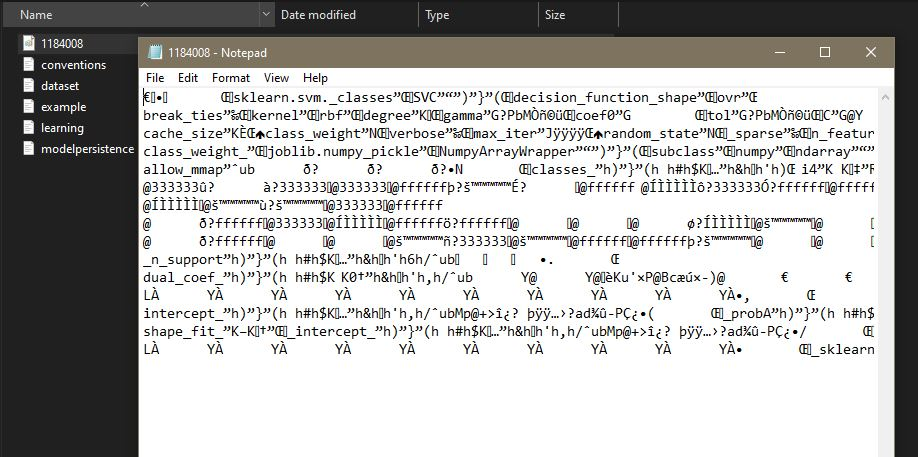
\includegraphics[width=.8\textwidth]{figures/1184008/chapter1/4b.JPG}
    \end{center}
   
    \item mencoba Model persistence, dengan membuka link sebelumnya dan mencari persistence, lalu buat file baru pada spyder dan run
    \begin{center}
    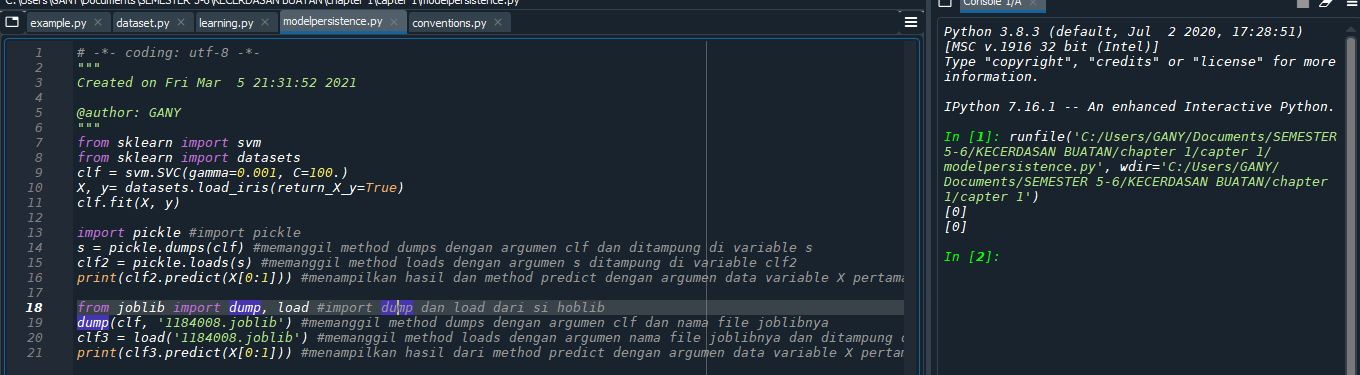
\includegraphics[width=.8\textwidth]{figures/1184008/chapter1/mo.JPG}
    \end{center} 
    SC : ModelPrecistensi
    \begin{verbatim}
    from sklearn import svm
    from sklearn import datasets
    clf = svm.SVC(gamma=0.001, C=100.)
    X, y= datasets.load_iris(return_X_y=True)
    clf.fit(X, y)
    import pickle
    s = pickle.dumps(clf) 
    clf2 = pickle.loads(s)
    print(clf2.predict(X[0:1])) 
    from joblib import dump, load 
    dump(clf, '1184008.joblib')
    clf3 = load('1184008.joblib') 
    print(clf3.predict(X[0:1]))    
    \end{verbatim}
    \item Mencoba Conventions, dengan membuka link sebelumnya dan mencari convestion, lalu buat file baru pada spyder dan run
     \begin{center}
    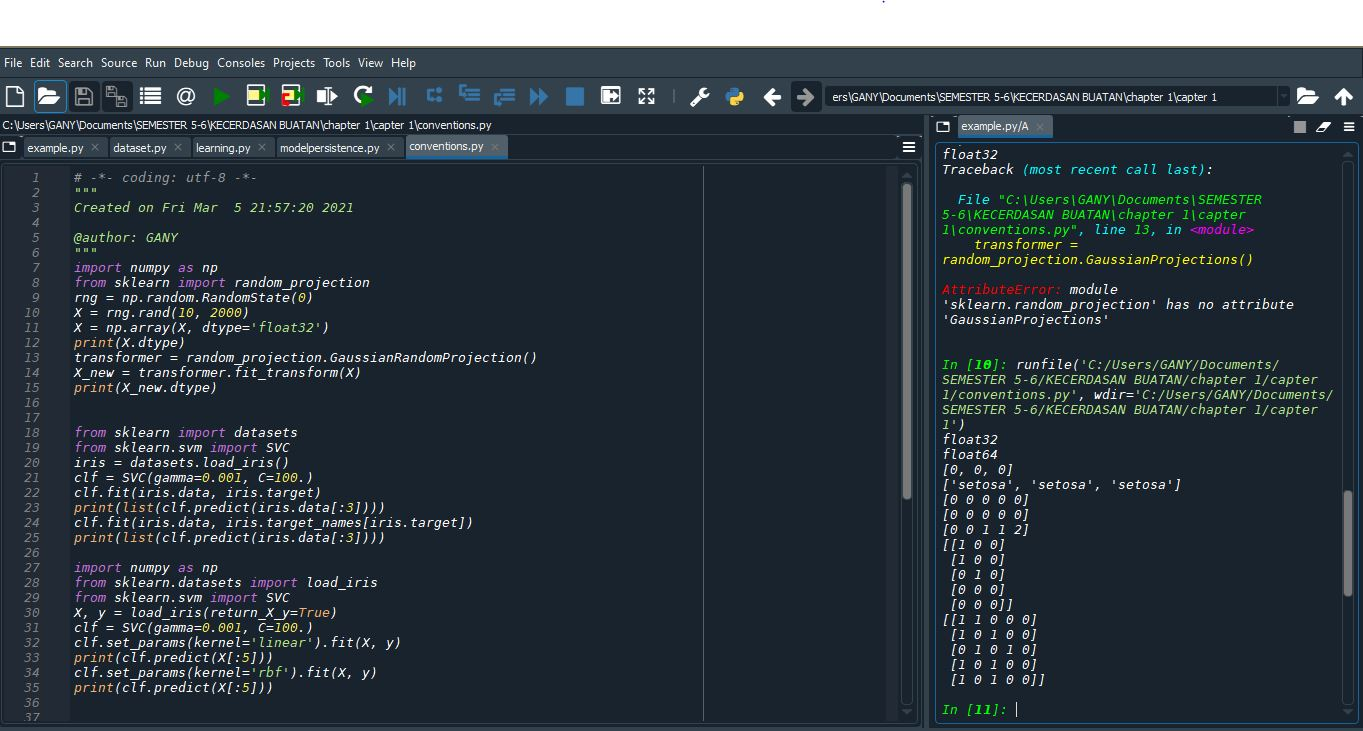
\includegraphics[width=.8\textwidth]{figures/1184008/chapter1/6.JPG}
    \end{center}
    Sc : Conventions
    \begin{verbatim}
    import numpy as np
    from sklearn import random_projection
    rng = np.random.RandomState(0)
    X = rng.rand(10, 2000)
    X = np.array(X, dtype='float32')
    print(X.dtype)
    transformer = random_projection.
    GaussianRandomProjection()
    X_new = transformer.fit_transform(X)
    print(X_new.dtype)
    from sklearn import datasets
    from sklearn.svm import SVC
    iris = datasets.load_iris()
    clf = SVC(gamma=0.001, C=100.)
    clf.fit(iris.data, iris.target)
    print(list(clf.predict(iris.data[:3])))
    clf.fit(iris.data, iris.target_names[iris.target])
    print(list(clf.predict(iris.data[:3])))
    import numpy as np
    from sklearn.datasets import load_iris
    from sklearn.svm import SVC
    X, y = load_iris(return_X_y=True)
    clf = SVC(gamma=0.001, C=100.)
    clf.set_params(kernel='linear').fit(X, y)
    print(clf.predict(X[:5]))
    clf.set_params(kernel='rbf').fit(X, y)
    print(clf.predict(X[:5]))    
    \end{verbatim}
\end{enumerate}

\section{Error dan Penanganannya}
\begin{enumerate}
    \item Terdapat error dalam learning.py yaitu dataseat is not define
      \begin{center}
    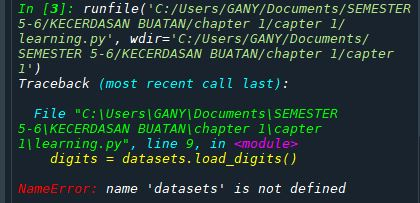
\includegraphics[width=.8\textwidth]{figures/1184008/chapter1/error 2.JPG}
    \end{center}
    \item kode eror dan jenis errornya
    NameError: name 'datasets'is not defined, dimana datasets tidak terdefinisi karena tidak diimport
    \item penangananya adalah harus adanya pendefinisian dari dataseats dengan import dataseats pada sklearn. sehingga kan menghasilkan hasil seperti yang diinginkan. dan perhatikan agar tidak terjadi typo atau kekurangan titik koma
    
\end{enumerate}

